\section{Design \& User Interface}

This section details the design considerations that were made prior to constructing the user interface; it demonstrates the four main components of the user interface and the issues encountered during creation.

\subsection{Design Considerations}
When implementing the user interface, we wanted to ensure that the design of the application was consistent with the Android 4.0 design ideology. To achieve this, we referenced the Android design and style guide which outlines some of the key aspects of an Android 4.0 application, and some of Google's design decisions made throughout the OS, which should be implemented and considered within our application. This included decisions such as universal behaviour of the back button, how preferences should be handled within the application using a separate fragment or activity, and interaction and navigation of the different subactivities of our application. 

Later versions of Android make use of an Actionbar which is implemented across all Android 4.0 applications as a way of providing a consistent method for navigation. This has therefore been included within the application with a main logo and icons which can be used to navigate between the different viewpoints.

For the implementation of the UI, it was designed so there were different activities for the different viewpoints available. There was one main activity for the home screen, and then activities for the map, graph, leaderboard, and the settings were implemented using the newer preference fragment class, which would match the preferences theme of the system. We implemented the "Up" navigation option only on settings, as it is the only part of the application that is not a top level activity. Therefore all of the other activities make use of the back navigation instead, due to the lack of a hierarchy between the different viewpoints. Tapping on the logo in the top left corner will always take you back to the default home view.

There are certain key design principles that have been outlined by Google in their style guide, that we have tried to implement within the application. Making sure that the important information is easily accessible, and the most important options and features can be accessed from the main home screen, providing an overview of events and the next time they should take caffeine. In the app structure they stress how the main home view should not just be a navigation menu, but instead stating the importance of "making content the centerpiece of your start screen", which this satisfies.

\subsection{Final Design}

\subsubsection{Action Bar}
\begin{figure}[ht]
\begin{center}

\includegraphics[scale=1]{images/actionbar.png}
\caption{Action Bar} 
\end{center}
\end{figure}

The action bar has used well known and explanatory symbols to illustrate each activity that the buttons relate to (e.g a map of the world for maps, and the well known settings wrench symbol). The colours used are contrasting so that the symbols show up clearly for the user. 

\newpage
\subsubsection{Activities}

Below is a figure detailing the main screens of each activity section in Opticaff. 

\begin{figure}[ht]
\begin{center}
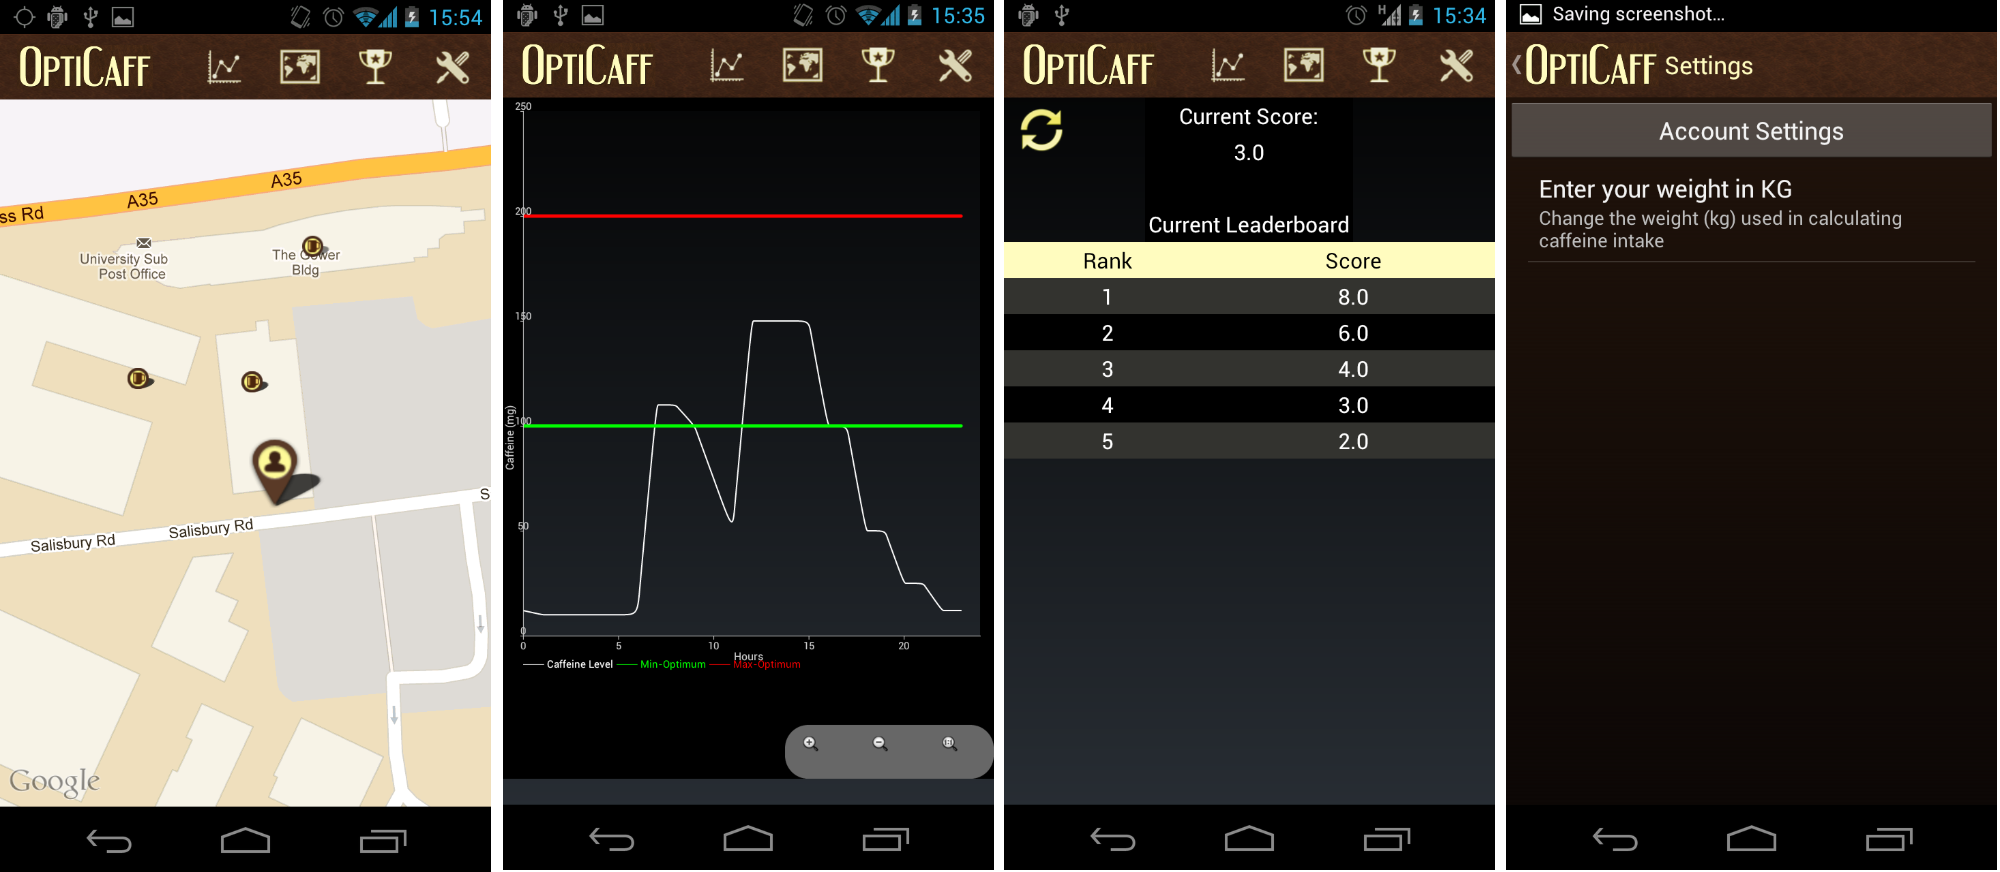
\includegraphics[scale=0.23]{images/app.png}
\caption{Activities: Maps, Graphs, Leaderboard \& Settings} 
\end{center}
\end{figure}

\textbf{(a) Map Screen} \newline
This screen uses the well known pointers utilised in popular map applications such as google maps to illustrate the users location. The nearest caffeine vendors are shown in small brown circles around the map to give the user a visual idea of their proximity.

\textbf{(b) Graph Screen} \newline
This screen shows the tracking of a users caffeine levels. This enables the user to easily see if they are staying within optimal levels. The colours red and green are used for dangerous and optimal levels respectively. This is an intuative design choice as red is often used to portray danger or stop signals wheras green is used for positive symbols such as in traffic lights. 

\textbf{(c) Leaderboard Screen} \newline
This screen allows users to see their current score and to compare it with those of their friends. Putting the users score at the top in large text allows them to immediately assess whether they are achieveing a good score through the use of positive and negative symbols. 

\textbf{(d) Settings Screen} \newline
This screen allows users to change their settings. It is currently very simplistic as the prototype has minimal settings. However it provides a basic explanation for the setting to aid the user in why they would edit it. 

\subsection{Issues with User Interface}
When developing the UI, we were initially implementing the different activities in fragments, with one main container activity managing all of them. Unfortunately this caused issues when we implemented the map, as due to some incompatibilities between the MapActivity class in android and the new Fragment classes, there were problems when trying to contain what was viewed as an activity, within a fragment. This meant that we implemented the different parts of the application as different activities.
